\documentclass[border=2mm]{standalone}

\usepackage{pgfplots}
\pgfplotsset{compat=1.18}
\usetikzlibrary{arrows.meta, calc, positioning, decorations.pathreplacing, calligraphy}

\usepackage{xcolor}
\definecolor{den-1}{HTML}{111111}   % Đen #111111
\definecolor{den-2}{HTML}{222222}   % Đen #222222
\definecolor{den-3}{HTML}{333333}   % Đen #333333
\definecolor{den-4}{HTML}{444444}   % Đen #444444
\definecolor{den-5}{HTML}{555555}   % Đen #555555
\definecolor{den-6}{HTML}{666666}   % Đen #666666

\tikzset{
  >=Stealth,
  originlabel/.style={
    font=\small\sf,
    anchor=north east, 
    yshift=-0.1ex,     
    xshift=-0.1ex      
  }
}
\usepgfplotslibrary{fillbetween}

\begin{document}
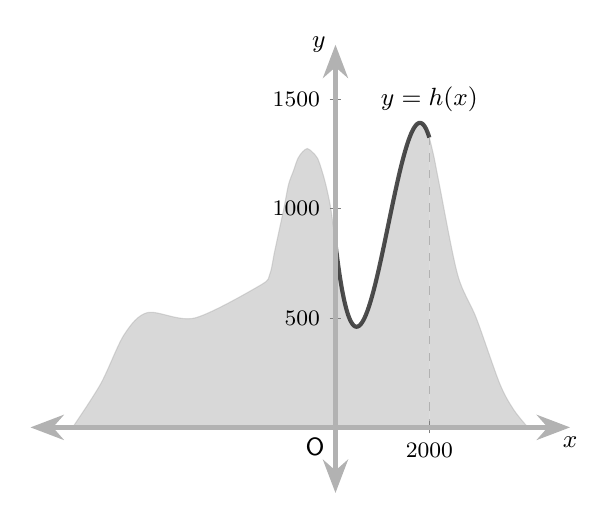
\begin{tikzpicture}
\begin{axis}[
    axis on top,
    font=\small\sf,
    axis lines=middle,
    axis line style={<->, line width=2pt, color=den-6!50},
    xlabel=$x$, ylabel=$y$,
    xlabel style={below, font=\small\sf},
    ylabel style={left, font=\small\sf},
    xmin=-6500, xmax=5000,
    ymin=-300, ymax=1750,
    xtick={2000},
    ytick={500,1000,1500},    
    tick label style={font=\footnotesize\sf, /pgf/number format/use comma=false, /pgf/number format/1000 sep={}},
    clip=false, 
]

\node[originlabel] at (axis cs:0,0) {O};

\addplot[
  name path=h,
  domain=0:2000, 
  samples=200, 
  restrict y to domain=-1000:2000,
  unbounded coords=discard, 
  line width=1.5pt, 
  color=den-2, 
  opacity=.8] 
    {(-1/1320000)*x^3+(9/3520)*x^2-(81/44)*x+840};

\path[name path=axis] (0,0) -- (2000,0);

\addplot [
  fill=den-6!50,
  opacity=.5,
  draw=none
] fill between [
  of=h and axis
];

\draw [dashed, color=den-6!50] (2000,0) -- (2000,1325);

\node at (2000,1400) [anchor=south] {\small $y=h(x)$};

\addplot [
  name path=h-1,
  color=den-6!50,
  opacity=.5,
  smooth
  ] coordinates {
  (2000,1325)
  (2100,1235) 
  (2200,1125) 
  (2600,700) 
  (3000,500)
  (3500,200)
  (3800,80)
  (4100,0)
  };

\path[name path=axis-1] (2000,0) -- (4100,0);

\addplot [
  fill=den-6!50,
  opacity=.5,
  draw=none
] fill between [
  of=h-1 and axis-1
];

\addplot[
    name path=h-2,
    smooth,
    color=den-6!50,
    opacity=.5
  ] coordinates {
    (0,840)
    (-100,1000)
    (-190,1095)
    (-270,1160)
    (-380,1230)
    (-500,1260)
    (-600,1275)
    (-700,1260)
    (-800,1230)
    (-900,1170)
    (-1000,1110)
    (-1100,1000)
    (-1200,900)
    (-1300,800)
    (-1400,700)
    (-1600,650)
    (-3000,500)
    (-4000,525)
    (-4500,425)
    (-5000,200)
    (-5600,0)
  };

\path[name path=axis-2] (-5600,0) -- (0,0);

\addplot [
  fill=den-6!50,
  opacity=.5,
  draw=none
] fill between [
  of=h-2 and axis-2
];

\end{axis}
\end{tikzpicture}
\end{document}
